%課題研究レジュメテンプレート ver. 1.2

\documentclass[uplatex]{jsarticle}
\usepackage[top=20mm,bottom=20mm,left=20mm,right=20mm]{geometry}
\usepackage[T1]{fontenc}
\usepackage{txfonts}
\usepackage{wrapfig}
\usepackage[expert,deluxe]{otf}
\usepackage[dvipdfmx,hiresbb]{graphicx}
\usepackage[dvipdfmx]{hyperref}
\usepackage{pxjahyper}
\usepackage{secdot}

\makeatletter
  \renewcommand{\section}{%
    \if@slide\clearpage\fi
    \@startsection{section}{1}{\z@}%
    {\Cvs \@plus.5\Cdp \@minus.2\Cdp}% 前アキ
    {.5\Cvs \@plus.3\Cdp}% 後アキ
    %{\normalfont\Large\headfont\raggedright}}
    {\normalfont\raggedright}}

  \renewcommand{\subsection}{\@startsection{subsection}{2}{\z@}%
    {\Cvs \@plus.5\Cdp \@minus.2\Cdp}% 前アキ
    {.5\Cvs \@plus.3\Cdp}% 後アキ
    %{\normalfont\large\headfont}}
    {\normalfont}}

  \renewcommand{\subsubsection}{\@startsection{subsubsection}{3}{\z@}%
    {\Cvs \@plus.5\Cdp \@minus.2\Cdp}%
    {\z@}%
    %{\normalfont\normalsize\headfont}}
    {\normalfont}}
\makeatother
%ここから上を編集する必要はない.





\title{\vspace{-14mm}ソーシャルゲームにおける登録数の増加と稼働日数の推移の関連性について}
\author{PMコース 矢吹研究室 1342029 遠藤一輝}
\date{}%日付を入れる必要はない.
\pagestyle{empty}%ページ番号は振らない.
\begin{document}
\maketitle





\section{研究の背景}

ゲームの開発技術が進歩していくにつれ,ゲームの種類も多様化してきている.その中の一形態として最近急激に数を増やした分野にソーシャルゲームがある.スマートフォンの性能の向上により本格的なゲームの動作にも耐え,携帯電話はゲーム機としての側面も持つようになった.ソーシャルゲーム黎明期には複雑な操作を必要としない単純なゲームが多かったが,携帯電話の処理機能の向上によってゲーム内容もより複雑なものへとなっていった.\par
規模の拡大は凄まじい速度で進行しており,2007年にわずか4億円であった市場が2008年には48億円となった.2009年には235億円とさらに数を伸ばし,その後も2010年には1067億円,2011年には2000億円以上とその勢いはとどまることを知らない\cite{shinbun}.%引用1
だがその隆盛の裏には多くの失敗や挫折があり,様々な事情によりサービスを停止したゲームが多くある.\par
ソーシャルゲームが成功したかどうかを判断する指標の一つとして登録人数がある.ソーシャルゲームを運営する上で登録人数は常に意識していかなければならない.
しかし,ソーシャルゲームの数が増え生存競争が激しくなった昨今では,顧客を掴むためにゲームを魅力的なものにしていく必要がある.
そのために登録人数の増加の傾向を分析し,分析の結果を元に現状を改善していく事は重要である.



\section{研究の目的}

ソーシャルゲームの登録人数と稼働日数の推移を調査し,パターンの分類をする.
各パターンを分析し,分析の結果を見ることで現行のソーシャルゲームにおける今後の登録人数の推移を予測する.




\section{プロジェクトマネジメントとの関連}

以下の点からプロジェクトの成功率を高めることができる.

\begin{enumerate}
\item 登録人数の推移を分析することで,現在登録人数はどの様な推移をしているのかがわかり,推移の状況にあった対策を講じやすくなる.
\item 登録人数増加のための手段を用いた時点のグラフの変化を見ることで,どの様な手段が多く登録人数を伸ばしやすいのかということを予測できる.
\end{enumerate}


\section{研究の方法}

\subsection{可視化の方法}


公式による発表が行われたソーシャルゲームから,一定登録数到達時の人数と日時を抜き出し,その推移を可視化する.稼働日数は稼働開始日から一定登録人数到達日までの日数とする.
可視化されたグラフから登録人数の増加の傾向をパターンに分類する.



\subsection{条件}


抜き出すソーシャルゲームの条件は以下のものとする.
\begin{enumerate}


\item 11月20日時点までにサービスが開始している.
\item 一定登録人数到達時に公式によるアナウンスがされる.

\end{enumerate}


\subsection{サンプルの選出方法}

データのサンプルの選出についてはネットランキング\cite{octba}\cite{appget}の1位から10位までを抜き出し,出てきたゲームの中からソーシャルゲームのみを対象とする.ソーシャルゲームの抽出を数十週にわたって行う.抽出されたソーシャルゲームの中から無作為にサンプルを選出する.




\begin{wrapfigure}[10]{r}{13cm}
\vspace*{-\intextsep}
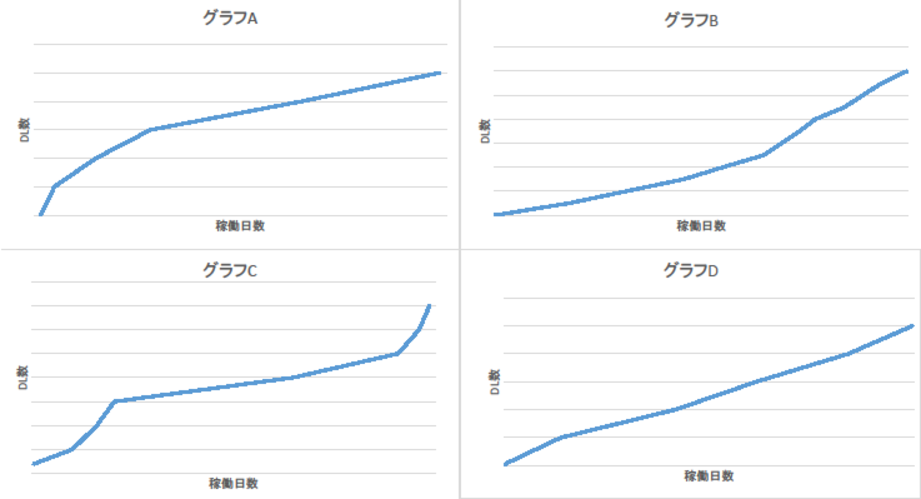
\includegraphics[width=11cm,clip]{g1.pdf}
\label{サンプル図}
\end{wrapfigure}


\section{現在の進捗状況}

分析のデータサンプルとして38件のソーシャルゲームを調査し,登録人数と稼働日数の推移について可視化を行った.可視化したグラフの傾向を元に,4つのパターンに分類した.


\begin{enumerate}
\item グラフA:
サービスの開始直後に急激に登録人数が伸び,以降傾きが緩やかになるパターンである.
ビッグタイトルや稼働前の情報から期待の集まる作品に多く見られた.
一方で稼働後のイメージとのギャップなどで登録人数が伸びきらず,失速するパターンもあった.

\item グラフB:
サービス開始からしばらくは緩やかな傾きが続くが,とある時点を境に傾きが急激に上昇するパターンである.ふとしたきっかけで知名度が上昇し,その後も人気を保ち続ける後天的にビッグタイトルとなった作品の傾向である.開始直後は知名度が少ないので,プレイヤーの作品に対するイメージが固まりづらい.知名度が高くなって以降は安定して高い伸び方を続けることが多い.

\item グラフC:
不規則に急激な上昇と緩やかな上昇を繰り返すパターンである.
ある程度の知名度がある作品とのコラボレーションなどによって急激に数を伸ばすが,その効果が薄れるにつれ上昇率も減衰し,しだいに傾きが緩やかになっていく.
その後別の案で同じサイクルを繰り返すため,不規則な推移になると考えられる.

\item グラフD:
平均的に登録人数を伸ばし続けるパターンである.
サービス開始から大きな変化をせず,安定して登録者数を伸ばし続ける.


\end{enumerate}







\section{今後の計画}

以下のように研究を進める計画である.

\begin{enumerate}
\item データの件数を増やし,データの信頼性の向上を図る.
\item グラフの推移を分類した4パターンについて,分析を行う.
\item 現行のゲームの現時点までのグラフの推移をみることで,そのゲームの今後の登録人数の推移を予測する.
\item 登録人数の今後の推移の予測の試行回数を増やし,予測の精度の向上を図る.
\end{enumerate}


\bibliographystyle{junsrt}
\bibliography{biblio}%「biblio.bib」というファイルが必要.

\end{document}